\documentclass[tikz]{standalone}
\renewcommand*{\familydefault}{\sfdefault}
\usepackage{standalone}
\usepackage{amssymb}
\usetikzlibrary{decorations}
%\usetikzlibrary{arrows.meta, decorations.pathmorphing, decorations.pathreplacing, shapes.geometric}
\usetikzlibrary{bayesnet}

\begin{document}
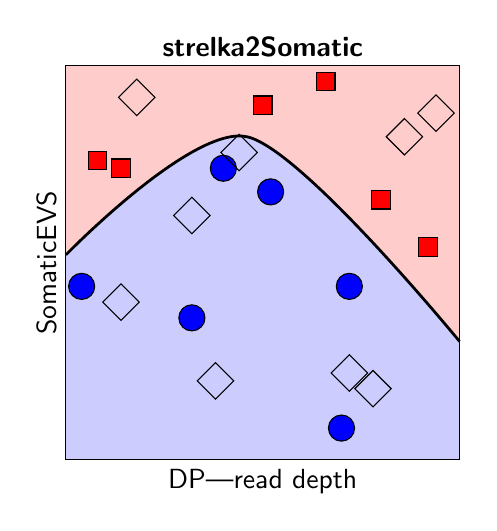
\begin{tikzpicture}%[font=\footnotesize, xscale=1.5]
% plot
% coordinates
\coordinate (SW) at (0,0);
\coordinate (NW) at (0,5);
\coordinate (SE) at (5,0);
\coordinate (NE) at (5,5);
\path (SW) -- node[rotate=90, anchor=south] {SomaticEVS} (NW);
\path (SW) -- node[anchor=north] {DP---read depth} (SE);
\path (NW) -- node[anchor=south] {\textbf{strelka2Somatic}} (NE);

\node (D1) at (0,2.6) {};
\node (D2) at (2.3,4.1) {};
\node (D3) at (5.0,1.5) {};



% filter
\fill[fill=red!20!white] (SW) rectangle (NE);
\fill[fill=blue!20!white] plot[smooth] coordinates {(D1) (D2) (D3)} -- (SE) --
(SW) -- (D1) -- (D3) -- (D1);
\draw[line width=1pt] plot[smooth] coordinates {(D1) (D2) (D3)};

% labeled points
% plot axes
\draw (SW) rectangle (NE);

% true positives
\begin{scope}[every node/.style={draw, rectangle, fill=red}]
\node at (0.4,3.8) {};
\node at (0.7,3.7) {};
\node at (3.3,4.8) {};
\node at (2.5,4.5) {};
\node at (4.0,3.3) {};
\node at (4.6,2.7) {};
\end{scope}

% false positives
\begin{scope}[every node/.style={draw, circle, fill=blue}]
\node at (0.2,2.2) {};
\node at (2.0,3.7) {};
\node at (3.5,0.4) {};
\node at (2.6,3.4) {};
\node at (3.6,2.2) {};
\node at (1.6,1.8) {};
\end{scope}



% unlabeled points
\begin{scope}[every node/.style={draw, diamond}]
\node at (0.7,2.0) {};
\node at (1.6,3.1) {};
\node at (3.9,0.9) {};
\node at (2.2,3.9) {};
\node at (1.9,1.0) {};
\node at (3.6,1.1) {};
\node at (4.7,4.4) {};
\node at (4.3,4.1) {};
\node at (0.9,4.6) {};
\end{scope}


\end{tikzpicture}
\end{document}
